\section{Results}
\label{sec:results}

We evaluate token pruning across six VLA models spanning three connector families on LIBERO-Object~\cite{liu2023libero} (10 tasks, 50 episodes each, 500 total). All success rates report Wilson 95\% confidence intervals for single-seed results and mean $\pm$ standard deviation for multi-seed results.

\subsection{Taxonomy Overview}
\label{sec:taxonomy_overview}

Table~\ref{tab:taxonomy} organizes seven models into four response classes. The taxonomy reveals that effective vision-to-LLM pipeline complexity, not the nominal connector label or model scale, is strongly associated with pruning tolerance. Token importance CV tracks this ordering continuously across an 8$\times$ parameter range (450M to 7B): uniformly critical models cluster at CV $< 0.06$, threshold-graded at $\sim$0.15, smooth graded at $\sim$0.22, and catastrophic cliff at $>$0.3. A pairwise comparison between $\pi_0$ and OpenVLA (both consuming 256 SigLIP-based~\cite{zhai2023siglip} tokens but differing in connector, backbone, and encoder fusion) yields a 63\,pp gap at $k{=}0.1$; this gap is consistent with the monotonic CV-degradation pattern across all seven models (Section~\ref{sec:linear_results}).

The four classes differ qualitatively in their failure mode. Uniformly critical models ($\pi_0$, $\pi_0.5$~\cite{black2025pi05}) distribute importance so evenly that no scoring method can identify dispensable tokens; pruning either preserves random spatial coverage (and survives) or removes a clustered patch (and fails). Threshold-graded models (X-VLA) tolerate removal up to a sharp onset point. Smooth graded models (OpenVLA, OFT, CogACT) degrade proportionally to the fraction removed. Catastrophic cliff models (SmolVLA) collapse at any removal level.

\begin{table*}[t]
\centering
\small
\caption{Seven-model connector taxonomy. CV = coefficient of variation of vision token L2 norms. $^\dagger\pi_0$: offline metrics only, no closed-loop evaluation; the 63\,pp gap vs.\ OpenVLA at $k{=}0.1$ mixes offline loss with closed-loop SR. $^\ddagger$X-VLA uses a linear projection followed by a 12-layer BART encoder; the effective pipeline is not purely linear. $^\S$OFT reports attention entropy and CV only (no pruning evaluation); both metrics match OpenVLA, consistent with the connector being associated with token importance structure. $^\|$CogACT: literature result from EfficientVLA~\cite{yang2025efficientvla}, not our evaluation.}
\label{tab:taxonomy}
\begin{tabular}{llcrcll}
\toprule
Model & Connector & Params & Tokens & CV & Representative Result & Class \\
\midrule
$\pi_0$~\cite{black2024pi0} & Linear proj & 3.3B & 256 & 0.038 & $k{=}0.1$: $\mathcal{L}_1{=}0.976$ ($+$2.4\%)$^\dagger$ & Uniformly critical \\
$\pi_0.5$~\cite{black2025pi05} & Linear proj ($\times\!\sqrt{d}$) & 4B & 768 & 0.055 & $k{=}0.5$: L2$=$33.4\%, R$=$69.4\% ($\Delta{=}$+36pp) & Uniformly critical \\
X-VLA~\cite{zheng2025xvla} & Linear + BART (12L)$^\ddagger$ & 880M & 50 & 0.151 & $k{=}0.9$: $97.8{\pm}0.4$, $k{=}0.85$: $67.9{\pm}0.3$ & Threshold-graded \\
OpenVLA~\cite{kim2024openvla} & 3-layer MLP & 7B & 256 & 0.215 & $k{=}0.5$: 37.4\% SR ($-$49\%) & Smooth graded \\
OFT~\cite{kim2025openoft} & 3-layer MLP & 7B & 256 & 0.219 & CV $0.219 \approx 0.215$; Ent.\ $0.667 \approx 0.661$$^\S$ & Smooth graded \\
CogACT~\cite{li2024cogact} & MLP proj & -- & -- & -- & 74.2\% SR under 78\% prune$^\|$ & Smooth graded \\
SmolVLA~\cite{shukor2025smolvla} & Pixel-shuffle & 450M & 128 & 0.314 & $k{=}0.95$: 0\% SR & Catastrophic cliff \\
\bottomrule
\end{tabular}
\end{table*}

\subsection{Pixel-Shuffle: Catastrophic Cliff-Edge}
\label{sec:smolvla_results}

The SmolVLA baseline (bypass mode, all 128 vision tokens) achieves 44.8\% SR (224/500, CI [40.5\%, 49.2\%]).\footnote{The official SmolVLA result is 87.3\% SR with batch size 64 on 8 GPUs. Our reproduction uses a smaller batch due to compute constraints.} Every pruning configuration produces 0\% SR across seven configurations varying scoring (learned ACIS vs.\ random), retention ratio ($k \in \{0.50, 0.70, 0.90, 0.95\}$), and mechanism (zero-masking, true removal, token merging). The cliff persists regardless of checkpoint quality: the official SmolVLA HF checkpoint (57.2\%--59.2\% SR across two evaluation protocols; Appendix~\ref{app:smolvla_ablation}) also collapses to 0\% under random $k{=}0.95$ (5\% removal), L2 norm $k{=}0.9$ (10\% removal), and L2 norm $k{=}0.5$ (Table~\ref{tab:smolvla_ablation}). The failure is architectural, not a training artifact.

The pattern generalizes across LIBERO suites: Spatial 0.6\%, Goal 0\%. Pixel-shuffle folds each $4{\times}4$ patch block into a single token by channel concatenation; removing one token eliminates an entire $4{\times}4$ receptive field. The resulting spatial entanglement means even 5\% removal ($k{=}0.95$, losing 7 of 128 tokens) destroys task-critical visual information. Full ablation results appear in Table~\ref{tab:smolvla_ablation}, Appendix~\ref{app:smolvla_ablation}.

\subsection{MLP Projector: Smooth Graded Degradation}
\label{sec:openvla_results}

Under random token removal, OpenVLA degrades gracefully across all retention ratios: 74.0\% (baseline) $\rightarrow$ 69.4\% at $k{=}0.95$ ($-4.6$\,pp) $\rightarrow$ 62.0\% at $k{=}0.90$ $\rightarrow$ 49.0\% at $k{=}0.70$ $\rightarrow$ 37.4\% at $k{=}0.50$ $\rightarrow$ 20.6\% at $k{=}0.30$ (Figure~\ref{fig:degradation_curve}; full results with CIs in Table~\ref{tab:openvla_full}, Appendix).\footnote{A second random seed confirms the graded pattern: 62.2\% at $k{=}0.9$ ($+$0.2\,pp), 44.4\% at $k{=}0.7$ ($-$4.6\,pp), 35.6\% at $k{=}0.5$ ($-$1.8\,pp). All within 5\,pp of the primary seed. Per-seed details in Table~\ref{tab:openvla_multiseed}, Appendix~\ref{app:openvla_multiseed}.} At $k{=}0.30$, two tasks reach 0\% SR, but eight retain non-zero performance: degradation is graded, not cliff-edge. Random token removal provides a conservative lower bound on architectural resilience; learned scoring methods would likely yield better retention.

OFT~\cite{kim2025openoft} retains OpenVLA's MLP connector but replaces the action head; its attention entropy (0.667) matches standard OpenVLA (0.661). The connector, not the action head, is associated with token importance structure. EfficientVLA~\cite{yang2025efficientvla} corroborates the graded pattern from the literature: CogACT~\cite{li2024cogact} (MLP projector) retains 74.2\% SR under 78\% pruning.

To control for scoring method in cross-architecture comparisons, we evaluate L2 norm-based selection on OpenVLA. At moderate-to-aggressive retention ($k \leq 0.7$), L2 performs within 2--6\,pp of random removal\footnote{OpenVLA random results use seed$\,{=}\,$7; L2 norm results use seed$\,{=}\,$42. Same-seed (seed42) gaps: 5.4\,pp at $k{=}0.7$, 3.6\,pp at $k{=}0.3$ (21.4\% random vs.\ 25.0\% L2); same-seed at $k{=}0.5$: 35.8\% random vs.\ 39.2\% L2 (gap 3.4\,pp).} (Table~\ref{tab:openvla_l2_vs_random}, Appendix~\ref{app:l2_vs_random}). At $k{=}0.9$, L2 outperforms random by 8.6\,pp (70.6\% vs.\ 62.0\%, reproducible across two random seeds), consistent with the weak but non-zero importance gradient predicted by CV$\,{=}\,$0.215: the signal is exploitable only when few tokens are removed.

\subsection{Linear Projection: From Uniformly Critical to Threshold-Graded}
\label{sec:linear_results}

Three models share a linear projection connector yet exhibit qualitatively different pruning responses. The divergence traces to what happens \emph{after} the projection: nothing ($\pi_0$), a learned scaling ($\pi_0.5$), or a full 12-layer encoder (X-VLA).

\paragraph{$\pi_0$ (3.3B, 256 tokens, pure linear).} Offline normalized L1 action loss at $k{=}0.1$ is 0.976, a 2.4\% \emph{improvement} over the unpruned baseline.\footnote{Offline action loss measures single-step prediction quality; closed-loop evaluation may reveal additional degradation.} CV$\,{=}\,$0.038 indicates near-uniform token norms. Near-uniform L2 norms (CV$\,{=}\,$0.038) suggest that no token subset carries disproportionate information, so random removal approximates uniform spatial downsampling and the model compensates.

\paragraph{$\pi_0.5$ (4B, 768 tokens, linear $\times\!\sqrt{d}$).} The baseline achieves 98.2\% SR. This model reveals that low CV does not imply tokens are dispensable; it implies uniform criticality. The response is strongly method-dependent: random removal at $k{=}0.5$ retains 69.4\% SR ($-$28.8\,pp), while L2 norm-based removal at the same ratio collapses to 33.4\% ($-$64.8\,pp). The gap of 36\,pp is the largest method-dependent effect at $k{=}0.5$ in our study.

At $k \leq 0.7$, random removal degrades monotonically (77.2\%, 69.4\%, 36.4\% at $k{=}0.7, 0.5, 0.3$; seed43 within 1\,pp). At higher retention, a task-specific random cliff emerges on LIBERO-Object: SR drops from 69.4\% ($k{=}0.95$) to 5.0\% ($k{=}0.85$) before recovering to 77.2\% ($k{=}0.7$), a 72\,pp swing; the same $k{=}0.85$ on LIBERO-Spatial retains 58.4\% (Appendix~\ref{app:pi05_crosssuite}). L2 norm selection produces a V-shaped curve: 55.0\% at $k{=}0.7$, 33.4\% at $k{=}0.5$ (the valley), 51.0\% at $k{=}0.3$, confirmed across two seeds ($\sigma = 0.1$\,pp at the valley).\footnote{V-shape valley at $k{=}0.5$: 33.4\% (seed42) vs.\ 33.6\% (seed43), $\sigma{=}0.1$\,pp. V-depth: 17.6\,pp (seed42), 21.8\,pp (seed43). Full multi-seed table in Appendix~\ref{app:pi05_multiseed}.} The non-monotonic L2 pattern arises because norm ranking in a low-CV distribution selects spatially clustered tokens (slight norm variations correlate with image regions), and the resulting loss of spatial coverage peaks at intermediate budgets.

This result demonstrates that models showing offline pruning tolerance can exhibit severe closed-loop degradation. Low-CV tokens are uniformly critical, not uniformly dispensable. L2 norm-based selection systematically concentrates on spatially correlated tokens and loses coverage; random selection preserves the uniform spatial distribution that these architectures require.

\paragraph{X-VLA (880M, 50 tokens, linear + 12-layer BART).} The 99.2\% baseline is maintained at $k{=}0.95$ ($99.1 \pm 0.2$\%, 3 seeds) and $k{=}0.9$ ($97.8 \pm 0.4$\%) under L2 norm-based removal. A sharp cliff appears at $k{=}0.85$ ($67.9 \pm 0.3$\%, $-$31\,pp, 3 seeds), with non-monotonic recovery at $k{=}0.80$ ($89.0 \pm 0.7$\%, 3 seeds) before degradation resumes: $58.6 \pm 0.4$\% at $k{=}0.7$, $43.4 \pm 0.8$\% at $k{=}0.5$, $22.0 \pm 0.9$\% at $k{=}0.3$, $4.7 \pm 0.6$\% at $k{=}0.2$, and near-zero at $k{=}0.1$. The cliff at $k{=}0.85$ (retaining 42 of 50 BART-encoded tokens) is reproducible across seeds (std $\leq$ 1.6\,pp). The non-monotonic dip is task-specific: four tasks lose $\sim$50\,pp each while six remain unaffected (Table~\ref{tab:xvla_cliff_pertask}, Appendix~\ref{app:xvla_cliff}). Under random removal, X-VLA exhibits a plateau: $65.1 \pm 0.1$\% at $k{=}0.7$ and $64.0 \pm 1.6$\% at $k{=}0.3$ (3 seeds each), confirming that L2 norm-based selection ($22.0 \pm 0.9$\% at $k{=}0.3$) is far more destructive than random for this intermediate-CV architecture.

That this threshold appears under importance-based removal (the more favorable test) while OpenVLA degrades smoothly under random removal (the harder test) strengthens the architecture-dependent conclusion. The $\pi_0$--OpenVLA comparison (both consuming 256 SigLIP-based tokens, differing in connector, backbone, and encoder fusion) produces a 63\,pp gap at $k{=}0.1$, consistent with the connector-associated pattern observed across all seven models. This comparison involves differences in connector, backbone, and encoder fusion, limiting causal interpretation.

\subsection{VTR: Re-Encoding Overcomes Cliff-Edge}
\label{sec:smart_compress_results}

To test whether learned re-encoding can overcome the pixel-shuffle cliff-edge, we insert a 22.2M-parameter cross-attention module (Vision Token Re-encoder, VTR) between the vision connector and the LLM backbone (details in Appendix~\ref{app:smart_compress_details}). VTR compresses 128 input tokens to $M$ output tokens. Both VTR and the baseline train from the same SmolVLA-Base checkpoint for 100K steps with identical hyperparameters. An extended training control (same procedure without the compressor) achieves 45.0\% SR ($p > 0.9$ vs.\ the 44.8\% baseline); the gain is architectural, not from additional optimization steps.\footnote{The extended baseline also collapses to 0\% SR under pruning ($k{=}0.50$, random, true removal). Additional training does not mitigate the pixel-shuffle vulnerability.}

\begin{table}[t]
\centering
\small
\caption{VTR re-encoding vs.\ deletion on SmolVLA (LIBERO-Object). The M-curve is relatively stable: $M{=}16$ (87.5\% compression) matches $M{=}128$ (no compression) within 1.1\,pp. A parameter-matched MLP adapter achieves comparable SR ($p = 0.15$ vs.\ cross-attention). $^\ddagger$Mean $\pm$ std over 3 seeds (500 episodes each). Other rows: single seed with Wilson 95\% CI.}
\label{tab:smart_compress}
\begin{tabular}{lccrr}
\toprule
Method & $M$ & Red. & SR (\%) & Seeds \\
\midrule
\textit{Baseline} & 128 & 0\% & 44.8 & 1 \\
\textit{Ext.\ training} & -- & -- & 45.0 & 1 \\
\textit{Hard pruning} & -- & 50--90\% & 0.0 & mult. \\
\midrule
Cross-attn$^\ddagger$ & 16 & 87.5\% & 56.9$\pm$1.3 & 55.8/58.4/56.5 \\
Cross-attn$^\ddagger$ & 32 & 75\% & 60.1$\pm$1.3 & 61.6/59.2/59.6 \\
Cross-attn$^\ddagger$ & 64 & 50\% & \textbf{62.0}$\pm$2.3 & 61.6/60.0/64.4 \\
Cross-attn$^\ddagger$ & 96 & 25\% & 54.5$\pm$3.2 & 52.6/58.2/52.8 \\
Cross-attn$^\ddagger$ & 128 & 0\% & 58.0$\pm$3.5 & 59.8/54.0/60.2 \\
MLP adapter$^\ddagger$ & 32 & 75\% & 63.4$\pm$2.6 & 65.2/64.6/60.4 \\
\midrule
\multicolumn{5}{l}{\textit{Official checkpoint (59.2\% baseline)}} \\
Cross-attn & 32 & 75\% & 53.4 & 1 \\
\bottomrule
\end{tabular}
\end{table}

The M-curve is relatively stable (Table~\ref{tab:smart_compress}): $M{=}16$ (56.9\%, 87.5\% compression) performs within 1.1\,pp of $M{=}128$ (58.0\%, no compression). A parameter-matched MLP adapter achieves 63.4\% $\pm$ 2.6 at $M{=}32$ ($p = 0.15$ vs.\ cross-attention; Figure~\ref{fig:compression_curve}). Cross-suite evaluation confirms generalization: 53.2\% on LIBERO-Spatial and 56.4\% on LIBERO-Goal where hard pruning yields 0\% (Appendix~\ref{app:smart_compress_full}). VTR applied to OpenVLA yields 0\% SR even in passthrough mode: it is a targeted remedy for pixel-shuffle entanglement.

\subsection{CV Correlates with Optimal Pruning Strategy}
\label{sec:scaling_law}

Token importance CV correlates with both pruning tolerance and optimal strategy. Comparing L2 norm-based and random removal across three models, the gap $\Delta$(R$-$L2) decreases monotonically with CV at both $k{=}0.5$ and $k{=}0.7$ (full data in Table~\ref{tab:scaling_law}, Appendix~\ref{app:cv_scaling_table}). At $k{=}0.5$: $+$36.0\,pp ($\pi_0.5$, CV$\,{=}\,$0.055) $\rightarrow$ $+$26.9\,pp (X-VLA, CV$\,{=}\,$0.151) $\rightarrow$ $-$1.8\,pp (OpenVLA, CV$\,{=}\,$0.215). At $k{=}0.7$: $+$22.2\,pp $\rightarrow$ $+$6.5\,pp $\rightarrow$ $-$5.4\,pp. The monotonic ordering holds across a 2$\times$ change in token budget, indicating CV captures a structural property of the connector. Below CV $\approx 0.15$, L2 ranking captures spatial artifacts rather than importance; above it, importance-based scoring becomes beneficial (reversal at $k{=}0.3$; Appendix~\ref{app:cv_strategy_interaction}).

\begin{figure}[t]
\centering
\begin{subfigure}[b]{0.48\linewidth}
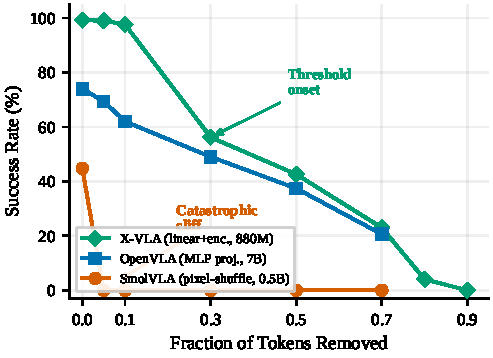
\includegraphics[width=\linewidth]{figures/paper/fig_degradation_curve.pdf}
\caption{Token pruning across connector classes.}
\label{fig:degradation_curve}
\end{subfigure}
\hfill
\begin{subfigure}[b]{0.48\linewidth}
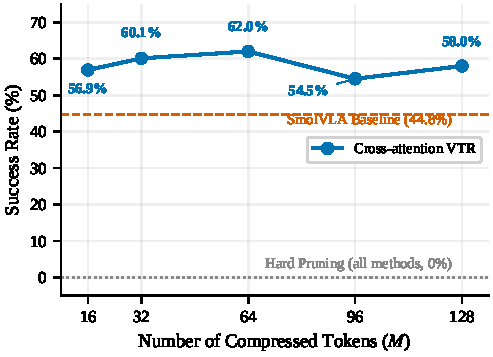
\includegraphics[width=\linewidth]{figures/paper/fig_compression_curve.pdf}
\caption{VTR M-curve and CV-strategy interaction.}
\label{fig:compression_curve}
\end{subfigure}
\caption{Token reduction on LIBERO-Object. (a)~Pruning: linear ($\pi_0$) uniformly critical, linear+encoder (X-VLA) threshold-graded, MLP (OpenVLA) smooth, pixel-shuffle (SmolVLA) collapses. (b)~VTR: $M{=}16 \approx M{=}128$ where deletion yields 0\%; CV-gap monotonic.}
\label{fig:results_combined}
\end{figure}

\enlargethispage{2\baselineskip}
\subsection{Cross-Suite Generalization}
\label{sec:cross_suite}

The cliff zone exhibits a suite $\times$ method interaction: at $k \in [0.85, 0.95]$, Object tasks collapse under random removal while Spatial tasks degrade gracefully (Figure~\ref{fig:crosssuite}, Table~\ref{tab:pi05_crosssuite}). L2 norm maintains a near-baseline plateau on both suites ($\leq 2.4$\,pp at $k \geq 0.85$). CV$\,{=}\,$0.055 correctly predicts this plateau on both suites despite qualitatively different cliff profiles, confirming CV as a model-level diagnostic. Token importance heatmaps reveal a center-high, edge-low spatial pattern (Figure~\ref{fig:token_heatmap}, Appendix~\ref{app:token_heatmap}), formalized by a hypergeometric model $H(N{=}768,\, C{=}106,\, T{=}7)$: cliff onset at $k{=}0.96$ (10\% collapse probability) narrows to $k{=}0.90$ (90\%), RMSE${=}$0.018 (Appendix~\ref{app:cliff_model}). The model captures onset sharpness at high retention but does not generalize to moderate retention ($k \leq 0.7$), where compensatory mechanisms may emerge (\S\ref{sec:analysis}). The cross-suite difference is driven by Object's concentrated criticality ($C{=}106$) versus Spatial's distributed pattern ($C \approx 5$).